% easychair.tex,v 3.1 2011/12/30
%
% Select appropriate paper format in your document class as
% instructed by your conference organizers. Only withtimes
% and notimes can be used in proceedings created by EasyChair
%
% The available formats are 'letterpaper' and 'a4paper' with
% the former being the default if omitted as in the example
% below.
%
\documentclass[procedia]{easychair}
%\documentclass[debug]{easychair}
%\documentclass[verbose]{easychair}
%\documentclass[notimes]{easychair}
%\documentclass[withtimes]{easychair}
%\documentclass[a4paper]{easychair}
%\documentclass[letterpaper]{easychair}

% This provides the \BibTeX macro
\usepackage{doc}
\usepackage{makeidx}
\usepackage[utf8]{inputenc}
\usepackage[T1]{fontenc}
\usepackage{amsmath}
\usepackage{amssymb}
\usepackage{subfig}


% In order to save space or manage large tables or figures in a
% landcape-like text, you can use the rotating and pdflscape
% packages. Uncomment the desired from the below.
%
% \usepackage{rotating}
% \usepackage{pdflscape}

% If you plan on including some algorithm specification, we recommend
% the below package. Read more details on the custom options of the
% package documentation.
%
% \usepackage{algorithm2e}

% Some of our commands for this guide.
%
\newcommand{\easychair}{\textsf{easychair}}
\newcommand{\miktex}{MiK{\TeX}}
\newcommand{\texniccenter}{{\TeX}nicCenter}
\newcommand{\makefile}{\texttt{Makefile}}
\newcommand{\latexeditor}{LEd}

\DeclareMathOperator*{\argmax}{arg\,max}
\DeclareMathOperator*{\argmin}{arg\,min}
\DeclareMathOperator{\sign}{sign}
\newtheorem{hypothesis}{Hypothesis}

\def\procediaConference{99th Conference on Topics of
  Superb Significance (COOL 2014)}

%\makeindex

%% Front Matter
%%
% Regular title as in the article class.
%
\title{Local Tuning in Peano Curves-based Global Optimization Scheme}

% \titlerunning{} has to be set to either the main title or its shorter
% version for the running heads. When processed by
% EasyChair, this command is mandatory: a document without \titlerunning
% will be rejected by EasyChair

\titlerunning{Local Tuning in Peano Curves-based \ldots}

% Authors are joined by \and. Their affiliations are given by \inst, which indexes into the list
% defined using \institute
%
\author{
    Vladislav V. Sovrasov%\thanks{Designed and implemented the class style}
}

% Institutes for affiliations are also joined by \and,
\institute{
  State University of Nizhny Novgorod,
  Nizhny Novgorod, Russia\\
  \email{sovrasov.vlad@gmail.com}
 }
%  \authorrunning{} has to be set for the shorter version of the authors' names;
% otherwise a warning will be rendered in the running heads. When processed by
% EasyChair, this command is mandatory: a document without \authorrunning
% will be rejected by EasyChair

\authorrunning{Sovrasov}

\begin{document}

\maketitle

\keywords{advanced numerical methods, deterministic global optimization, speedup of convergence, derivative-free algorithms}

\begin{abstract}
This paper considers one of the methods to account for the local information on the
objective function in  Lipschitz global optimization problems. In the course of solving
such problems, an issue arises regarding estimating the Lipschitz constant of the
objective function arises. According to the classic scheme, this constant is a single
estimate for the whole search domain. The method of accounting for local properties
is based on building estimates of Lipschitz constants for the search subdomains,
and has previously been investigated for the one-dimensional case. For solving
multidimensional problems, dimension reduction is applied. A multidimensional
optimization problem is reduced to a one-dimensional problem, for which the objective
function satisfies the Hölder condition. In this paper, the application of building
local Hölder constant estimates in reduced multidimensional optimization problems using
the same scheme as is used in one-dimensional Lipschitzian problems is considered.
\end{abstract}

%\setcounter{tocdepth}{2}
%{\small
%\tableofcontents}

%\section{To mention}
%
%Processing in EasyChair - number of pages.
%
%Examples of how EasyChair processes papers. Caveats (replacement of EC
%class, errors).


%------------------------------------------------------------------------------
\section{Introduction}
\label{sect:introduction}

One-dimensional-characteristical algorithms represent one class of widely-used
optimization algorithms \cite{optHandbook}. A number of schemes to reduce multidimensional problems
to one or more one-dimensional problems, i.e. the \textit{dimension-reduction} schemes
have been developed \cite{evolvents2013}, \cite{gergelGrishaginStringin2013}.
All these schemes can be efficiently parallelized \cite{optParallelBook}.
\par
In recent years, when building global optimization algorithms, increased attention
has been paid to accounting for the local properties of the objective function.
In the case of characteristical schemes, this approach allows a mixed algorithm
to be developed \cite{mixedAlg} and different estimates of Lipschitz constants to
be used in different search domains \cite{sergLocalTuningFirst}. Originally, the
latter approach had been proposed for one-dimensional problems, and this has also
been examined when carrying out a nested optimization scheme \cite{nestedLocal}.
In all these cases, this approach has proven to be efficient, having essentially
accelerated the convergence of the optimization methods. This paper considers generalizing
the method for building local estimates of Lipschitz constants in the case of Hölder
functions obtained when reducing multidimensional optimization problems.

%------------------------------------------------------------------------------
\section{Problem Statement}
\label{sect:problem}

The global optimization problem can be formulated as follows: to find the global minimum of an
\(N\)-dimensional function \(\varphi(y)\) in a hyperinterval
\(D=\{y\in R^N:a_i\leqslant x_i\leqslant{b_i}, 1\leqslant{i}\leqslant{N}\}\):
\begin{displaymath}
  \varphi(y^*)=\min\{\varphi(y):y\in D\}.
\end{displaymath}
In order to obtain an estimate of the global minimum from a finite number of function value computations,
 \(\varphi(y)\) is required to satisfy Lipschitz condition.
\begin{displaymath}
\label{lip}
|\varphi(y_1)-\varphi(y_2)|\leqslant L\Vert y_1-y_2\Vert,y_1,y_2\in D,0<L<\infty
\end{displaymath}
\par
The use of the evolvents \(y(x)\) i.e. the curves filling the space are a classic
dimension-reduction scheme for global optimization algorithms \cite{evolvents2013}.
\begin{displaymath}
\label{cube}
\lbrace y\in R^N:-2^{-1}\leqslant y_i\leqslant 2^{-1},1\leqslant i\leqslant N\rbrace=\{y(x):0\leqslant x\leqslant 1\}
\end{displaymath}
\par
Such a mapping allows the reduction of a problem stated in a multidimensional space
to solving a one-dimensional problem at the expense of worsening its properties.
In particular, the one-dimensional function \(\varphi(y(x))\) is not a Lipschitzian but a Hölderian function:
\begin{displaymath}
\label{holder}
|\varphi(y(x_1))-\varphi(y(x_2))|\leqslant H{|x_1-x_2|}^{\frac{1}{N}},x_1,x_2\in[0,1]
\end{displaymath}
where the Hölder constant \(H\) is related to the Lipschitz constant \(L\) by the relation
\begin{displaymath}
H=4Ld\sqrt{N},d=\max\{b_i-a_i:1\leqslant i\leqslant N\}
\end{displaymath}
\par
Therefore, not limiting the generality, one can consider the minimization of the
one-dimensional function \(f(x)=\varphi(y(x))\), with \(x\in[0,1]\) satisfying Hölder condition.
The issues of numerically building the mapping like a Peano curve and the corresponding
theory have been considered in detail in \cite{evolvents2013}. Here we would note that an evolvent
built numerically is an approximation to the theoretical Peano curve with a precision
of the order \(2^{-m}\) where \(m\) is the building parameter of the evolvent.

%------------------------------------------------------------------------------
\section{Description of the Algorithm}
\label{sect:algorithm}

The algorithm considered for solving the stated problem implies generating
a sequence of points \(x_k\), in which the values of the minimized function \(z_k = f(x_k)\)
are computed. Let us call the process of computating the function value
(including calulating an image \(y^k=y(x^k)\)) a trial, and the pair \((x^k,z^k)\) ---
the result of the trial. A set of the pairs \(\{(x^k,z^k)\}, 1\leqslant k\leqslant n\)
makes up the search information accumulated by the method after executing \(n\) steps.
\par
At the first iteration of the method, a trial is executed at an arbitrary internal
point \(x^1\) within the interval \([0,1]\). Let us assume \(n \geqslant 1\) iterations
of the method to be completed, during the course of which the iterations in \(k = k(n)\)
points \(x_i, 1\leqslant i\leqslant k\) have been performed. Then, the point \(x^{k+1}\)
of the search trial for the next \((k+1)\)th iteration is determined in accordance with the rules:
\par
Step 1. Renumber the points in the set \(X_k=\{x^1,\dotsc,x^k\}\cup\{0\}\cup\{1\}\),
which includes the boundary points of the interval \([0,1]\) as well as the points of
preceding trials, by the lower indices in order of increasing coordinate values  i.e.
\begin{displaymath}
0=x_0<x_1<\dotsc<x_{k+1}=1
\end{displaymath}
\par
Step 2. Assuming \(z_i=f(x_i),1\leqslant i\leqslant k\), compute the values
\begin{equation}
\label{step2}
\mu=\max_{1\leqslant i\leqslant k}\dfrac{|z_i-z_{i-1}|}{\Delta_i},
\begin{matrix}
    M =
    \left\{
    \begin{matrix}
    r\mu,\mu>0 \\
    1,\mu=0
    \end{matrix} \right.
    \end{matrix}
\end{equation}
where \(r>1\) is a predefined parameter for the method, and \(\Delta_i=(x_i-x_{i-1})^\frac{1}{N}\).
\par
Step 3. For each interval \((x_{i-1},x_i),1\leqslant i\leqslant k+1\), compute the
characteristics according to the formulae
\begin{equation}
\label{step3_1}
R(1)=2\Delta_1-4\dfrac{z_1}{M},R(k+1)=2\Delta_{k+1}-4\dfrac{z_k}{M},
\end{equation}
\begin{equation}
\label{step3_2}
R(i)=\Delta_i+\dfrac{(z_i-z_{i-1})^2}{M^2\Delta_i}-2\dfrac{z_i+z_{i-1}}{M},1<i<k+1.
\end{equation}
\par
Step 4. Select the interval \((x_{t-1}, x_t)\) such that
\begin{equation}
\label{step4}
t=\argmax_{1\leqslant i \leqslant k+1}R(i),
\end{equation}
i.e., the interval with the maximal characteristic.
\par
Step 5. Execute a new trial at point \(x_{k+1}\) computed according to the formulae
\begin{displaymath}
x_{k+1}=\dfrac{x_{t}+x_{t-1}}{2},t=1,t=k+1,
\end{displaymath}
\begin{equation}
\label{step5}
x_{k+1}=\dfrac{x_{t}+x_{t-1}}{2}-\sign(z_{t}-z_{t-1})\dfrac{1}{2r}\left[\dfrac{|z_{t}-z_{t-1}|}{\mu}\right]^N,1<t<k+1.
\end{equation}
\par
The algorithm is terminated if the condition \(\Delta_{t}\leqslant \varepsilon\) is fulfilled;
here \(\varepsilon>0\) is the predefined accuracy. As an estimate of the global optimum solution of the problem the values
\begin{equation}
f_k^*=\min_{1\leqslant i \leqslant k}f(x_i), x_k^*=\argmin_{1\leqslant i \leqslant k}f(x_i)
\end{equation}
are selected. The theoretical substantiation of this method is presented in \cite{strOptBook}, chapter 8.

%------------------------------------------------------------------------------
\section{Local Adaptive Estimate of Hölder Constant}
%\label{sect:algorithm}
As it is seen from the scheme of the algorithm, regardless of the local properties
of the optimized one-dimensional function, the same estimate of the Hölder
constant (\ref{step2}) is used to compute the characteristic of all intervals (\ref{step3_1}), (\ref{step3_2}).
In \cite{sergLocalTuningFirst}, it has been proposed to use different values of \(M\) (\(M\) is the same as in (\ref{step2}), (\ref{step3_1})) for each interval,
and also the efficiency of this approach has been shown in the case of optimizing
one-dimensional functions that satisfy the Lipschitz condition. In \cite{nestedLocal},
the application of the adaptive estimates of Lipschitz constants in the multidimensional
nested optimization scheme has been considered. For each interval, the local estimate of the
constant is an additive convolution of the ``global'' and ``local'' constants
(\(\gamma\) and \(\lambda\), correspondingly):
\begin{displaymath}
  \begin{array}{lr}
    \lambda_i=\max\{H_{i-1},H_i,H_{i+1}\} \\
    H_i=\frac{|z_i-z_{i-1}|}{\Delta_i} \\
    H^k=\max\{H_i:i=2,\dots ,k\} \\
    \gamma_i=H^k\frac{\Delta_i}{\Delta^{max}} \\
    \Delta^{max}=\max\{\Delta_{i}:i=2,\dots ,k\}
  \end{array}
\end{displaymath}
\begin{equation}
\label{additiveConv}
M_i=r\cdot \max\{H_i, \frac{1}{2}(\lambda_i+\gamma_i),\xi\}
\end{equation}
A small \(\xi\) is chosen to prevent the function from being constant over the search interval.
This variant of convolution does not depend on the parameter \(r\), however, the adaptive convolution:
\begin{equation}
\label{additiveAdaptiveConv}
M_i=r\cdot \max\{H_i, \frac{\lambda_i}{r}+\frac{r-1}{r}\gamma_i,\xi\}
\end{equation}
has been introduced in \cite{gergel2010} and detailed considered (in case of solving one-dimentional Lipschitzian problems) in \cite{sergLocalTuning} as well.
If it is known a priori that the optimized function has a complex shape with multiple
local minima, then the initial value of \(r\) is specified to be large enough to
result in the dominance of the ``global'' component \(\gamma\) in the adaptive convolution.

%------------------------------------------------------------------------------
\section{Hypothesis about Convergence}
%\label{sect:algorithm}
In \cite{sergLocalTuning}, a theorem is given on the convergence of the method in the
case of a Lipschitz objective function. However, as a rule, such statements are
true for Hölder metrics as well. Therefore, the following hypothesis is presumably true:

\begin{hypothesis}
Assume the objective function \(f(x)\) to  satisfy Hölder condition with finite
constant \(H > 0\), and let x be a limit point of \(\{x_k\}\) generated by the algorithm.
Then, the following assertions hold:
\begin{enumerate}
  \item If \(x\in(0;1)\), then convergence to \(x\) is a bilateral one i.e. there
  exists two infinite subsequences of \(\{x_k\}\) converging to \(x\): one from the
  left, the other from the right;
  \item \(f(x_k) \geqslant f(x)\) for all trial points \(x_k, k \geqslant 1\);
  \item If there exists another limit point \(x^* = x\), then \(f(x) = f(x^*)\);
  \item If the function \(f(x)\) has a finite number of local minima in \([0, 1]\),
  then the point \(x\) is a local optimum;
  \item (Sufficient conditions for convergence to a global minimizer). Let \(x^*\)
  be a global minimizer of \(f(x)\). If there exists an iteration number \(k^*\)
  such that for all \(k > k^*\) the inequality
  \(M_j(k) > H_j(k)\) holds, where \(H_j(k)\) is the Hölder constant for the interval
  \([x_{j(k)-1}, x_{j(k)}]\) containing \(x^*\), and \(M_{j(k)}\) is its estimate.
  Then, the set of limit points for the sequence \(\{x_k\}\) coincides with the set
  of global minimizers for the function \(f(x)\).
\end{enumerate}
\end{hypothesis}

The proof of this hypothesis requires further theoretical studies. It was not performed
as part of this present work. The convergence has only been established numerically.

%------------------------------------------------------------------------------
\section{Experimental Results}
\label{sect:experiments}

The experiments to evaluate the efficiency of the method with a local adaptive
estimate of the Hölder constant have been carried out using the two-dimensional
classes of Grishagin (\(F_{GR}\)) \cite{grishaginClass} and GKLS problems \cite{gklsClass}.
Each class includes 100 multiextremal functions. In all experiments, the evolvent was
built with the density \(m = 12\), the parameter \(\varepsilon\) in the termination criterion
was set to \(10^{-3}\). The parameter \(r\) was selected as low as possible, at which
the given method solves all problems of the class. The search step for \(r\) was \(0.1\).

\par
For clarity in illustrating the advantages of the local adaptive scheme for estimating
the constant \(H\), let us consider a particular example of the results obtained by the method.
In Figure \ref{fig:grish_isolines}, the level lines of a function from the \(F_{GR}\) class and
 the trial points executed by the method with a global estimate of the Hölder constant, and with
 the one estimated according to formula (\ref{additiveConv}) are shown. As can be seen from
 the figures, the method using a global estimate of the constant executed a large
 number of trials in the vicinity of the global minimizer (a total of 1,086 trials
 were executed) before the termination condition was satisfied, whereas the method
 with the local adaptive estimate converged much faster (a total of 385 trials
 were executed). The same situation occurs when optimizing a function from the
 GKLS class (Fig. \ref{fig:gkls_isolines}). The method using the global estimate of
 the constant executed 2,600 trials while the method using the local adaptive estimate only
 executed 1,190 trials.

\begin{figure}[ht]
    \centering
    \subfloat[global \(H\) estimation]{{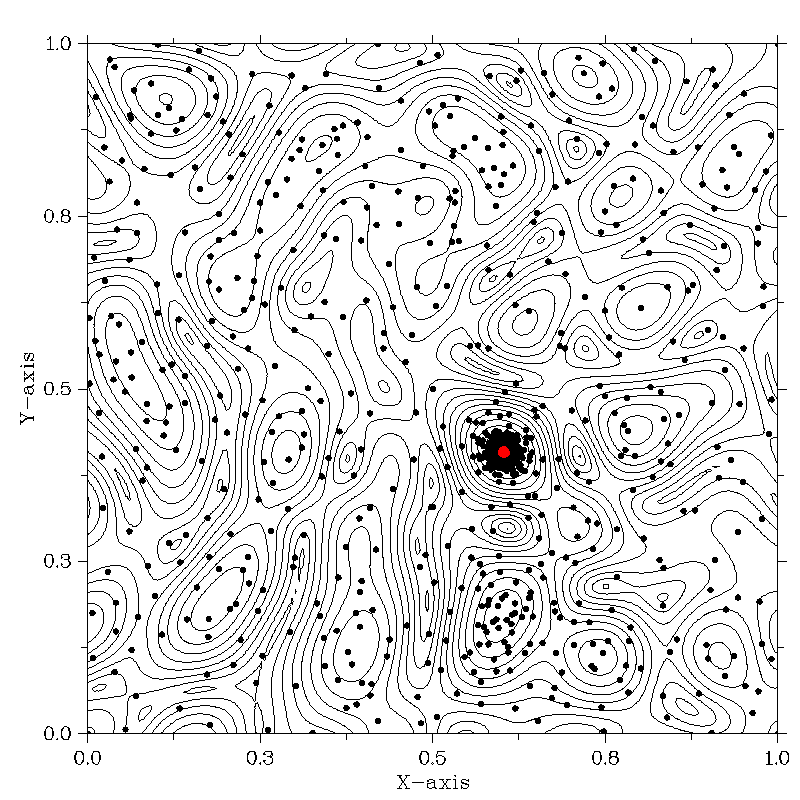
\includegraphics[width=0.45\textwidth]{images/gs_glob.png} }}
    \qquad
    \subfloat[local-adaptive \(H\) estimation]{{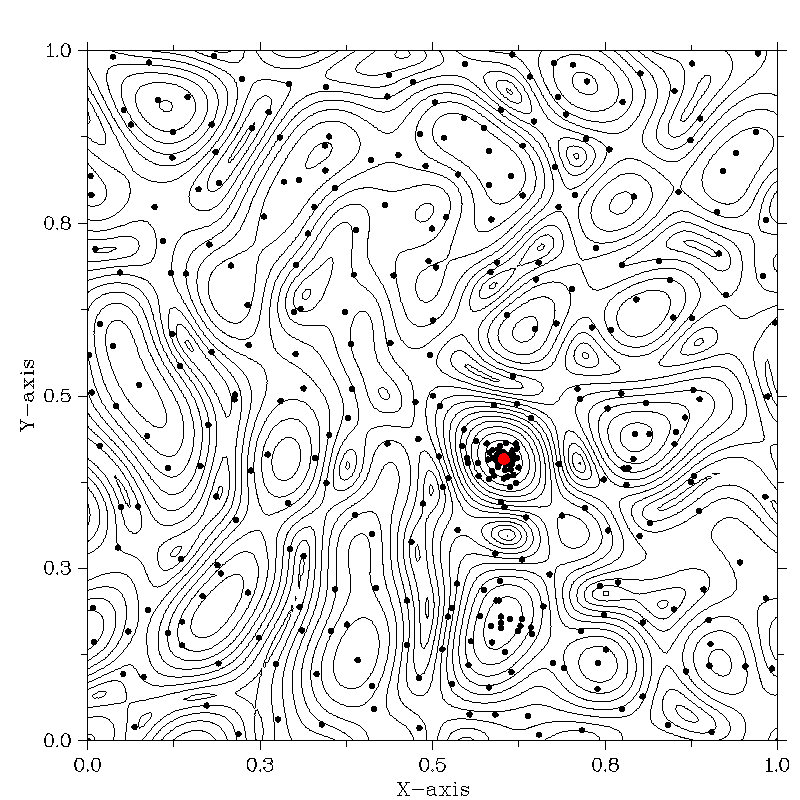
\includegraphics[width=0.45\textwidth]{images/gs_loc.png} }}
    \caption{The level lines of a function from \(F_{GR}\) class}
    \label{fig:grish_isolines}
\end{figure}

\begin{figure}[ht]
    \centering
    \subfloat[global \(H\) estimation]{{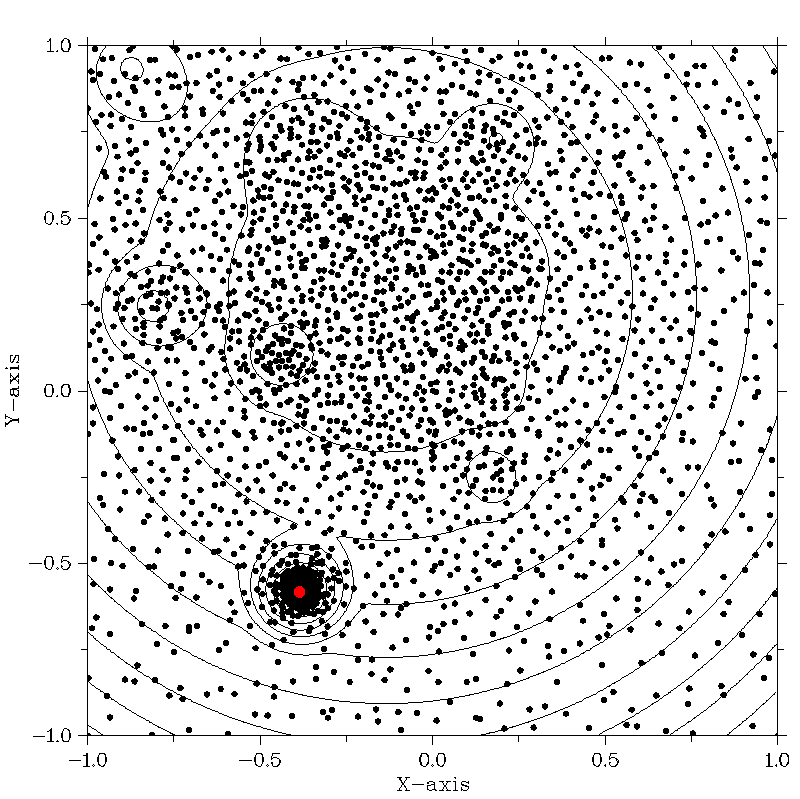
\includegraphics[width=0.45\textwidth]{images/gkls_glob.png} }}
    \qquad
    \subfloat[local-adaptive \(H\) estimation]{{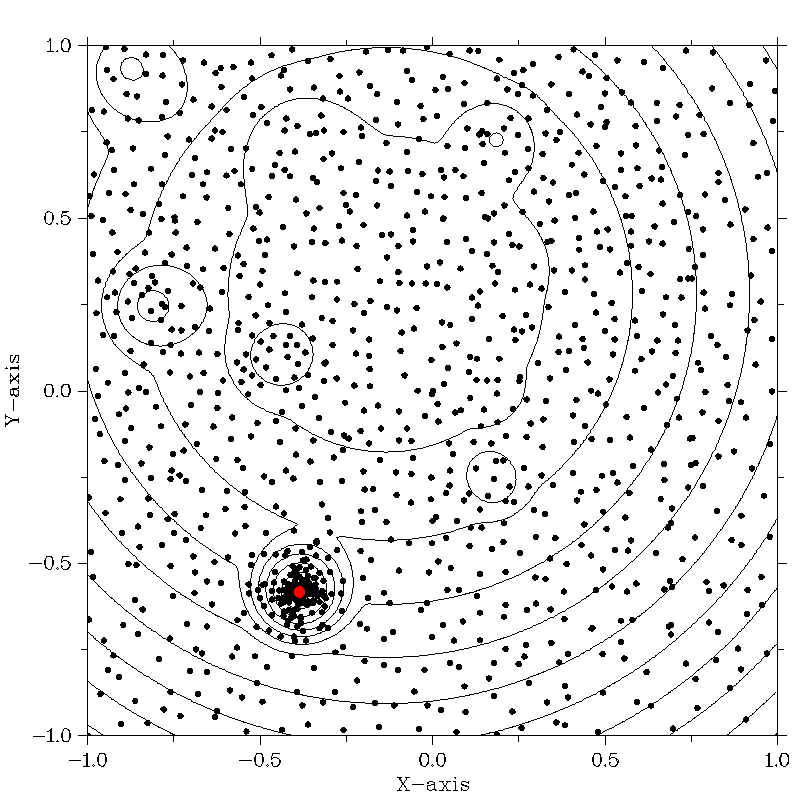
\includegraphics[width=0.45\textwidth]{images/gkls_loc.png} }}
    \caption{The level lines of a function from GKLS class}
    \label{fig:gkls_isolines}
\end{figure}
\par
Next, let’s compare the various alternatives for the method in the problem classes
considered. In order to evaluate the efficiency of an algorithm, we will use the
operating characteristics \cite{grishaginClass}, which are defined by a set of
points on the \((K, P)\) plane where \(K\) is the average number of search trials
conducted before satisfying the termination condition when minimizing a function
from a given class, and \(P\) is the proportion of problems solved successfully.
If at a given \(K\), the operating characteristic of a method goes higher than one
from another method, it means that at fixed search costs, the former method has a
greater probability of finding the solution. If some value of \(P\) is fixed, and the
characteristic of a method goes to the left from that of another method, the former
method requires fewer resources to achieve the same reliability.

\begin{figure}[ht]
  	\center
    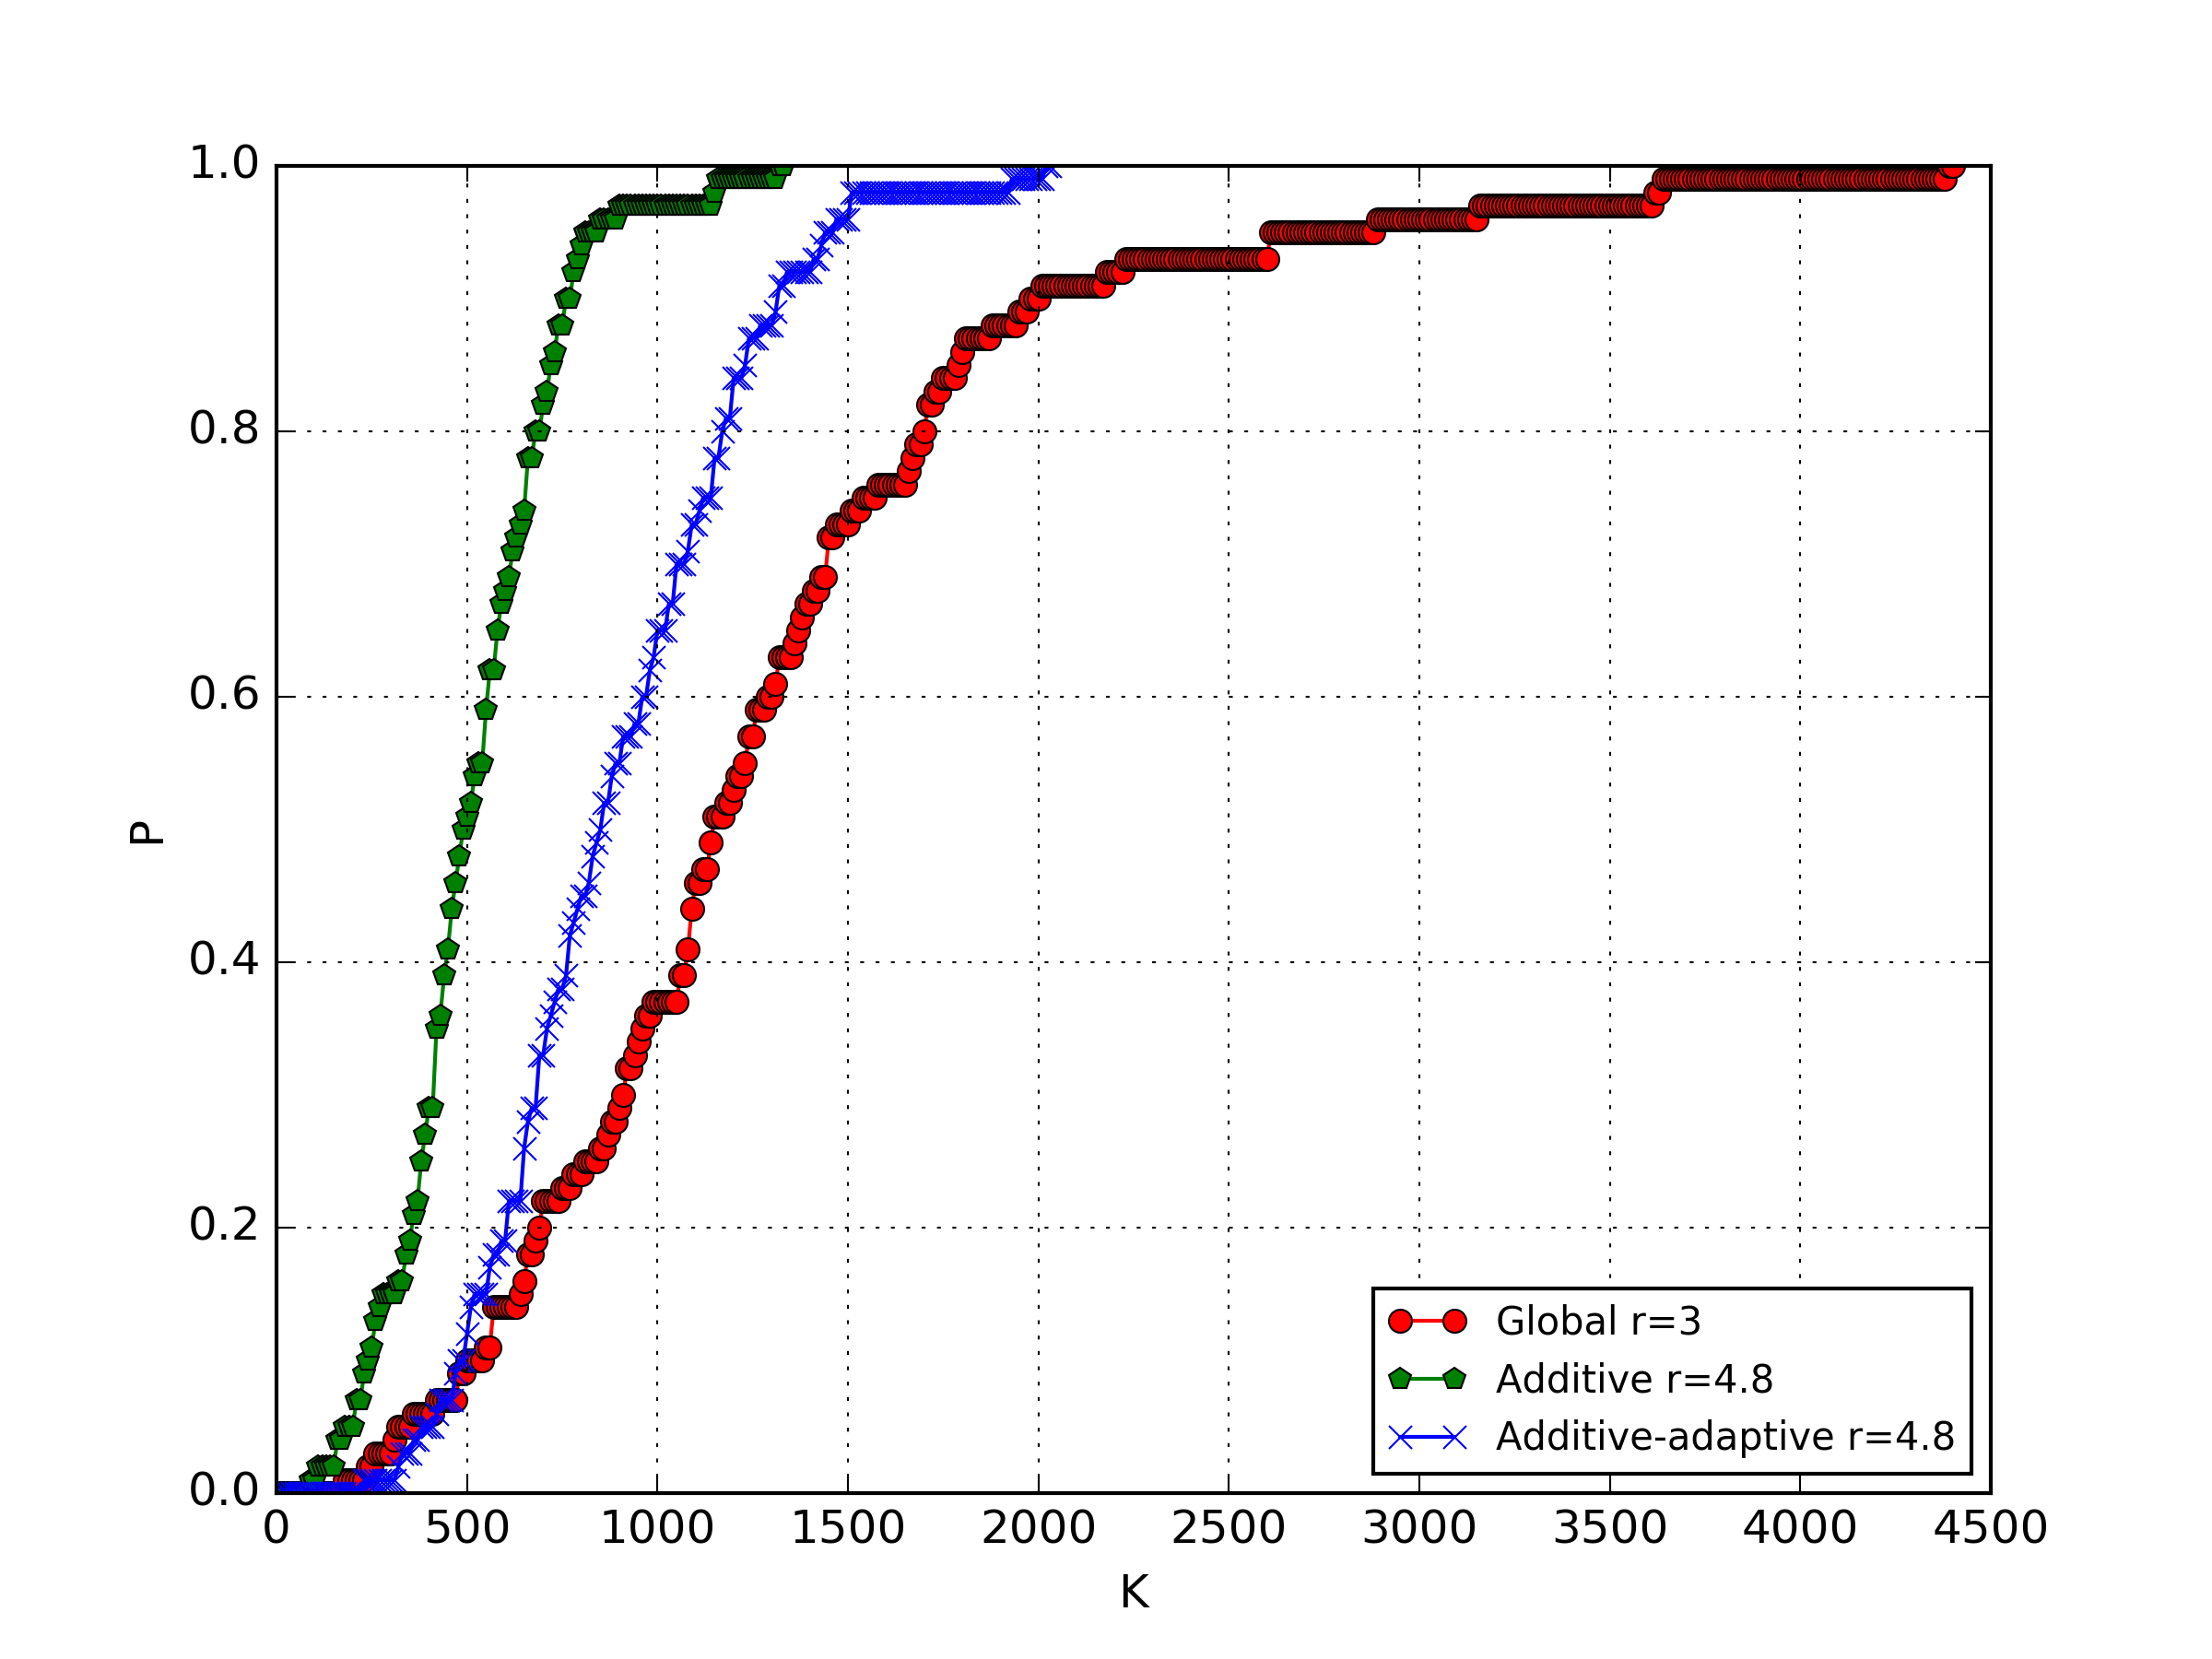
\includegraphics[width=0.75\textwidth]{images/grishagin.png}
    \caption{Operating characteristics of the methods compared on \(F_{GR}\) problems class}
    \label{fig:grishh_op}
\end{figure}
\par
As can be seen from the operating characteristics in Figures \ref{fig:grishh_op}
and \ref{fig:gkls_op}, both methods using a local adaptive estimate of the Hölder
constant have demonstrated an essential advantage. However, both methods require setting
a higher value for the parameter \(r\). If one compares the methods with both the
adaptive and non-adaptive convolution (\ref{additiveConv})(\ref{additiveAdaptiveConv}),
the advantage of the latter can clearly be seen, although it requires a higher value
for the reliability parameter \(r\) to solve problems from the GKLS class.

  \begin{figure}[ht]
  	\center
    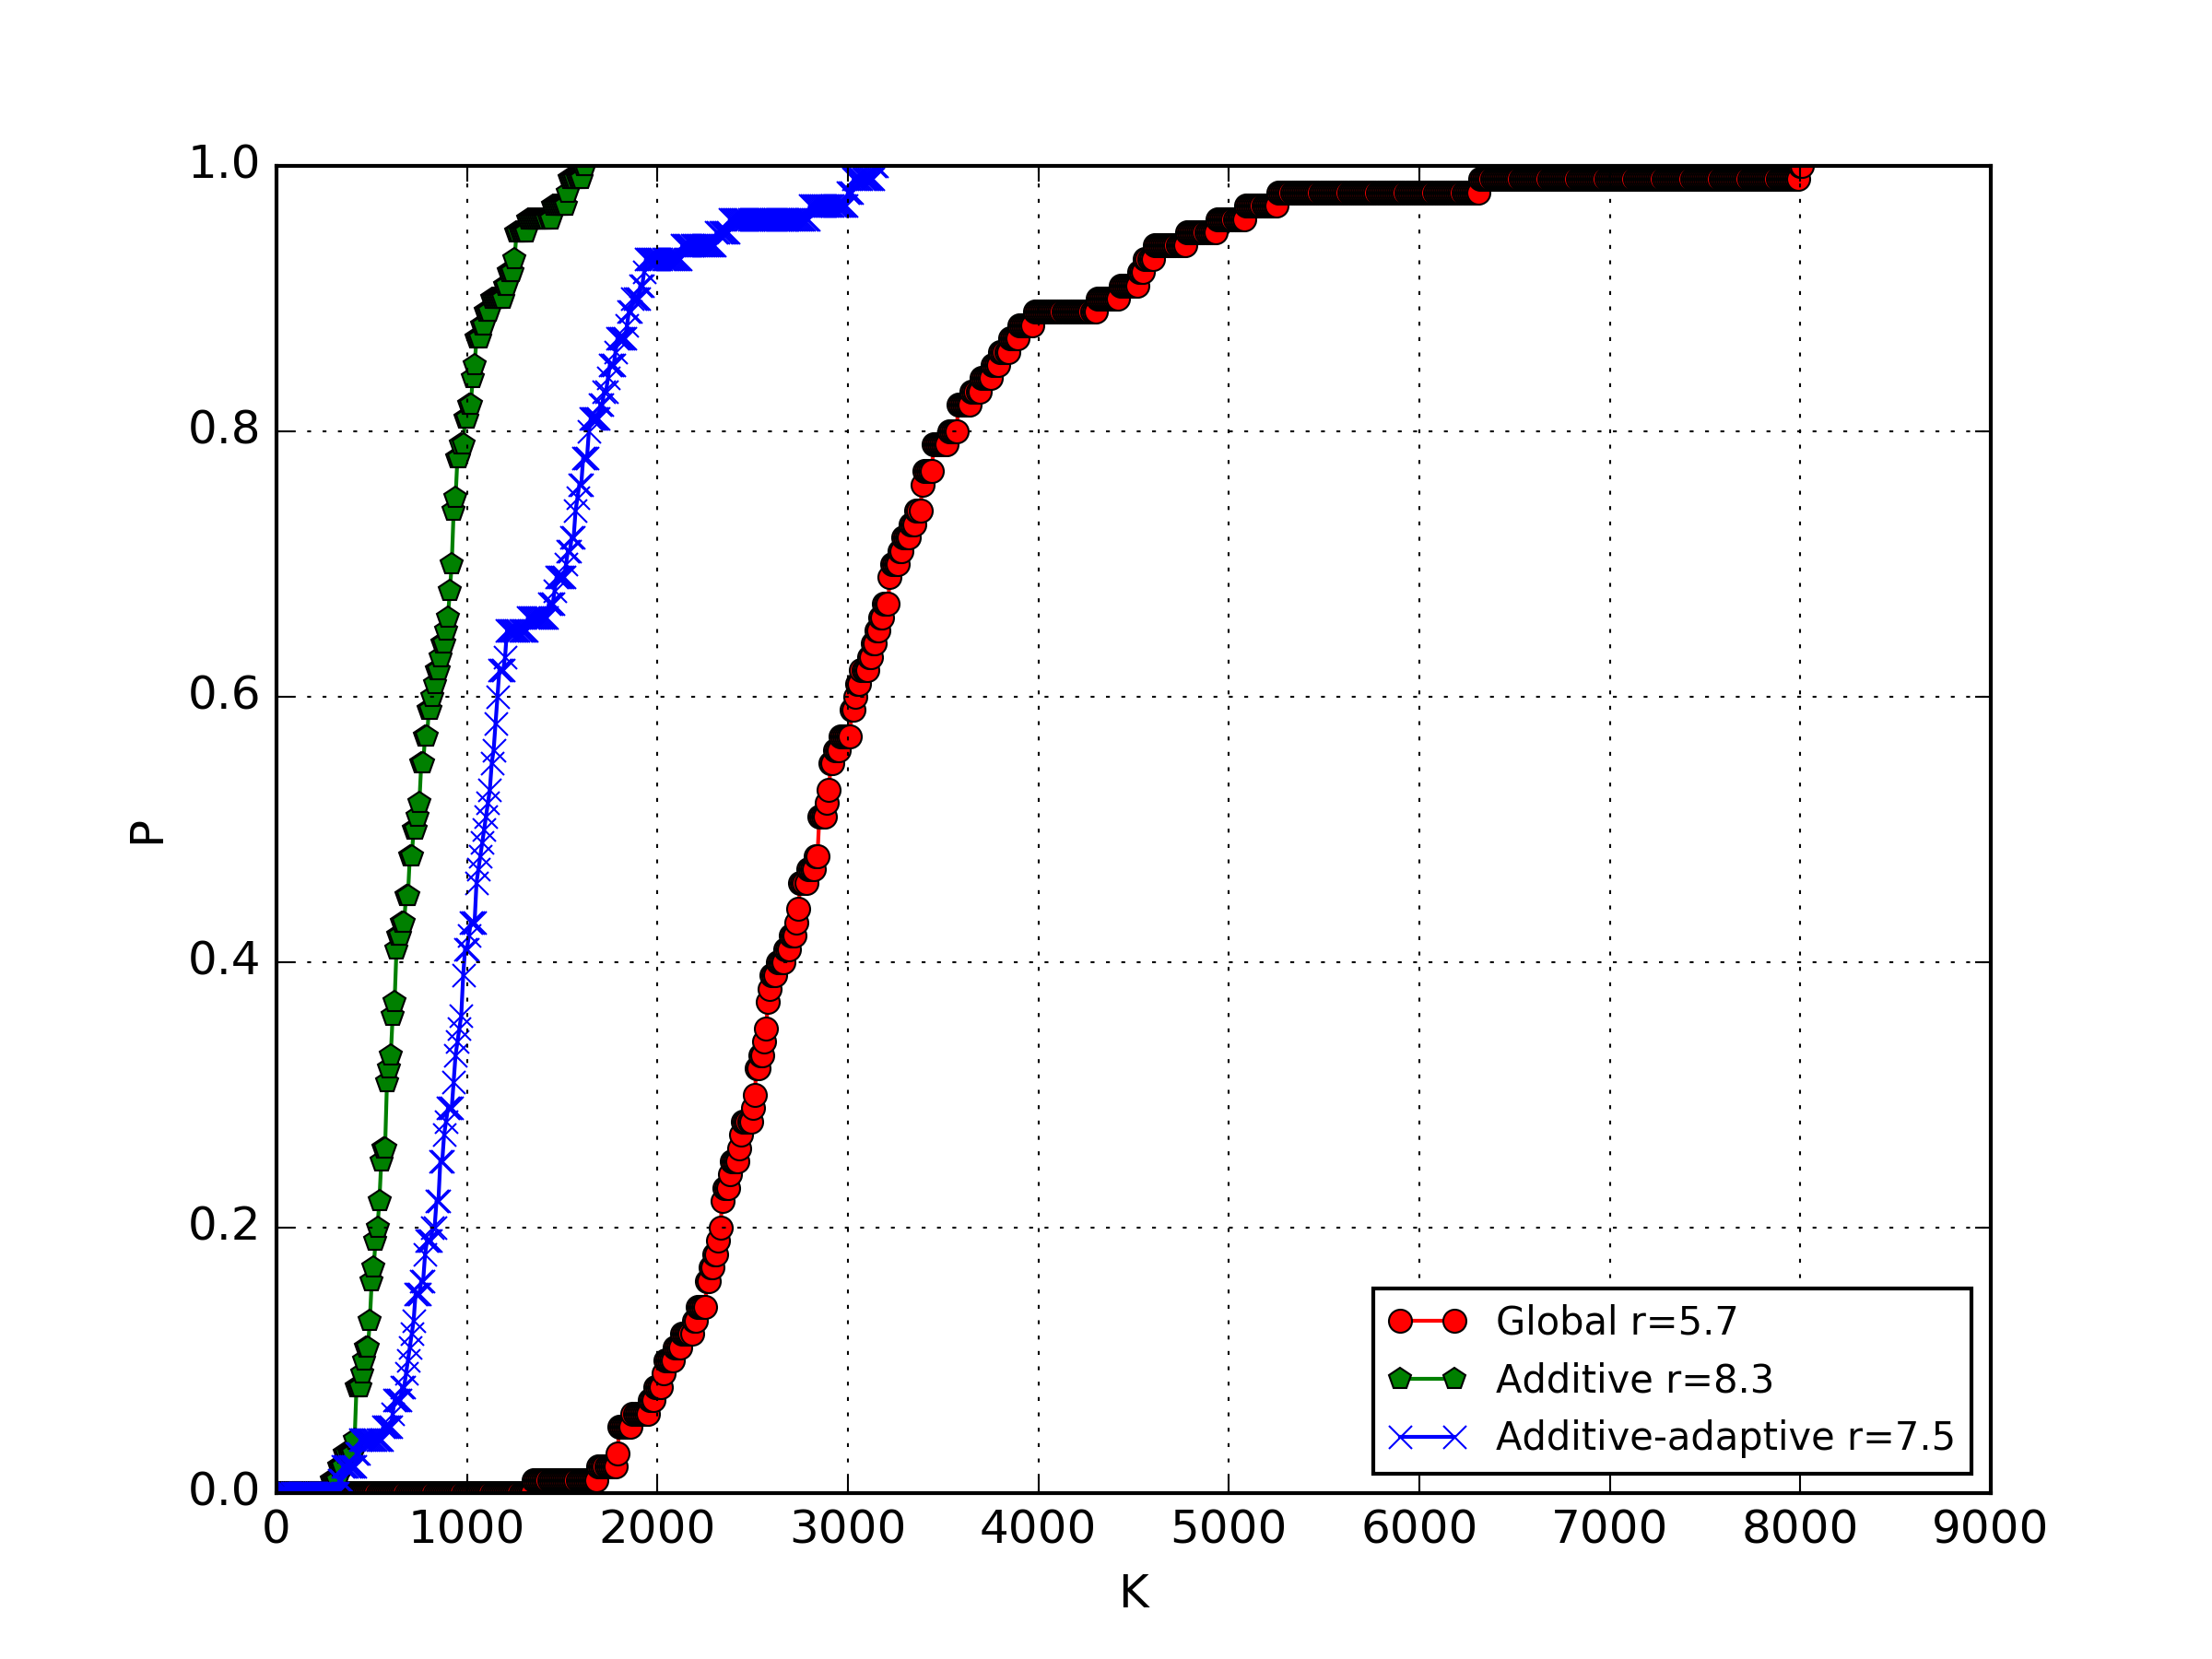
\includegraphics[width=0.75\textwidth]{images/gkls-s.png}
    \caption{Operating characteristics of the methods compared on GKLS problems class}
    \label{fig:gkls_op}
  \end{figure}
%------------------------------------------------------------------------------
\section{Conclusions}
This present work considers global optimization problems and the deterministic methods
for solving them. The relevance of solving this class of problems is defined by the
importance of the applications (optimal design, problems of parameter identification,
pattern recognition, signal processing, etc.). The multiextremal (global) optimization
methods are extremely computationally costly, since these require constructing and using
adaptive models of the objective function behavior according to the trial results
accumulated while executing the algorithm.
\par
This paper considers the application of a method to account for the local behavior
of the objective function within the multidimensional multiextremal optimization method.
This method has previously been applied to one-dimensional problems only. Taking into
account the local properties are implemented in using different estimates of Hölder
constant within different search domains. Thus, the process of solving the problem is
accelerated significantly by means of reducing the number of search trials.
\par
The comparison of two different schemes for constructing estimates of the Hölder
constant (\ref{additiveConv}), (\ref{additiveAdaptiveConv}) has revealed the advantage
of scheme (\ref{additiveConv}). However, a larger value for the reliability parameter \(r\)
in the search method might be required to use this scheme for solving certain problems.
When solving complex problems with a small area of attraction for the global extremum,
scheme (\ref{additiveAdaptiveConv}) is preferable for the greater reliability of this method.
The efficiency of the considered approach has been confirmed by solving the series of
multidimensional problems from two classes.

%------------------------------------------------------------------------------
\section{Acknowledgements}
This research was supported by the Russian Science Foundation, project No 16-11-10150
``Novel efficient methods and software tools for the time consuming decision- making problems
with using supercomputers of superior performance.''

%------------------------------------------------------------------------------
% Refs:
%
\label{sect:bib}
%\bibliographystyle{plain}
%\bibliographystyle{alpha}
\bibliographystyle{unsrt}
%\bibliographystyle{abbrv}
\bibliography{ysc_paper}

%------------------------------------------------------------------------------
% Index
%\printindex

%------------------------------------------------------------------------------
\end{document}

% EOF
